\documentclass{article}
\usepackage{graphicx}

%opening
%\title{}
%\author{}

\begin{document}
The Brandenburg Gate (German: Brandenburger Tor) is an 18th-century neoclassical triumphal arch in Berlin, and one of the best-known landmarks of Germany. It is built on the site of a former city gate that marked the start of the road from Berlin to the town of Brandenburg an der Havel.
(all text and figures from Wikipedia article on Brandenburg gate)

\begin{figure}
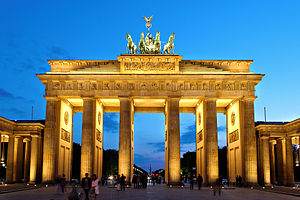
\includegraphics[width=0.6\textwidth]{Brandenburger_Tor_abends_from_wikipedia}

\caption{The Brandenburg gate}
\end{figure}

% an identical figure in both
\begin{figure} 
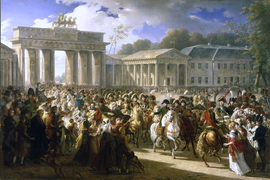
\includegraphics[width=0.5\textwidth]{270px-Charles_Meynier_-_Napoleon_in_Berlin}

\caption{Napoleon passing through the Brandenburg Gate after the Battle of Jena-Auerstedt (1806). Painted by Charles Meynier in 1810.}
\end{figure}
\end{document}

